\section{Performance Efficiency Focused Environements} \label{chapter3:software-performance}

With the limitations on performance presented in the previous section, both academy and industry communities proposed alternative solutions with performance in mind.
Section \ref{chapter3:software-performance:concurrency} presents the concurrent and parallel programming paradigms, and their programming models. % oriented on performance rather than maintainability.
Section \ref{chapter3:software-performance:adoption} presents the adoption steered by the performance efficiency of parallel programming.
Section \ref{chapter3:software-performance:maintainability-limitations} presents the consequences of parallelism on maintainability.
Finally, section \ref{chapter3:software-performance:summary} summarizes the three previous sections in a table.

\subsection{Concurrency} \label{chapter3:software-performance:concurrency}

\begin{figure}[h!]
\begin{center}
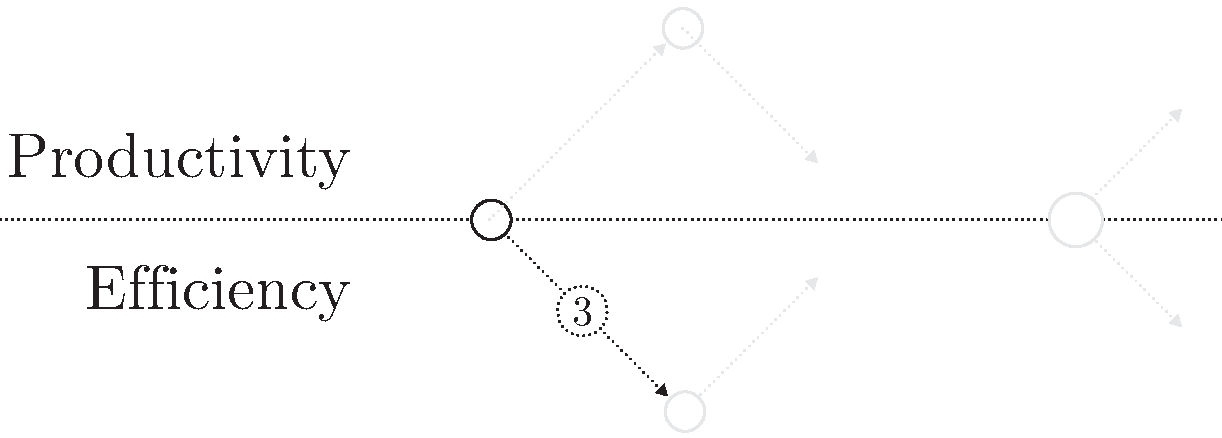
\includegraphics[width=0.6\textwidth]{../ressources/state-of-the-art-3.pdf}
\end{center}
\caption{}
\label{fig:state-of-the-art-3}
\end{figure}

Web servers need to be able to process huge amount of concurrent operations in a scalable fashion.
Concurrency is the ability to make progress on several operations roughly simultaneously.
It implies to draw boundaries in the memory to define independent regions, and causality in the execution to define independent tasks.
When both boundaries and causality are clearly defined, the tasks can be scheduled in parallel to make progress strictly simultaneously.

The definition of independent tasks allows the fine level synchronization within a task, and coarse level message passing between the tasks required for performence efficiency.
The synchronization of execution at a fine level assures the invariance on the shared state, and avoid communication overhead.
The message-passing at a coarser level assures the parallelism.
The two are indispensable for performance efficiency.

\subsubsection{Concurrent Programming} \label{chapter3:software-maintainability:concurrency:concurrent-programming}

% \cit{Building concurrent programming is like building a steam engine through a keyhole}{TODO}

\illustration{feu rouge et rond point}
Concurrent programming provides the mechanisms to define the causality of execution and assure the invariance of the global memory.
There are two scheduling strategies to execute tasks sequentially on a single processing unit, cooperative scheduling and preemptive scheduling.

\begin{description}
\item[Cooperative Scheduling] allows a concurrent execution to run until it yields back to the scheduler.
Each concurrent execution has an atomic, exclusive access on the memory.
\item[Preemptive Scheduling] allows a limited time of execution for each concurrent execution, before preempting it.
It assures fairness between the tasks, such as in a multi-tasking operating system.
But the unexpected preemption breaks atomicity, the developer needs to lock the shared state to assure atomicity and exclusivity.
\end{description}

The next paragraphs presents the event-driven programing model, based on cooperative scheduling, and the multi-threading programming model, based on preemptive scheduling.
Additionally, they present lock-free data-structures, which is independent from the scheduling strategy, as they rely on atomic memory operations.

\paragraph{Event-Driven Programming}

Event-driven execution model queues explicitly defined concurrent tasks needing access to shared resources.
The concurrent tasks are schedule sequentially to assure exclusivity, and cooperatively to assure atomicity.
% Web servers needs to be highly concurrent, and efficient.
It is very efficient for highly concurrent applications, as it avoids contention due to waiting for shared resources like disks, or network.
Several execution model rely on this execution model, like TAME \cite{Krohn2007}, Node.js\ftnt{https://nodejs.org/en/} and Vert.X\ftnt{http://vertx.io/}.
As well as some web servers like Flash \cite{Pai1999}, Ninja \cite{Gribble2001} thttpd\ftnt{http://acme.com/software/thttpd/} and Nginx\ftnt{https://www.nginx.com/}.

% However, a drawback of this model was that the execution context is lost at each event.
% The developer needs to explicitly transfer the relevant state to continue the execution from one event execution to another.

% + Fibers \cite{Adya2002}
% + Capricio \cite{Behren2003a} - User cooperative threads (also known as fibers / green threads)

% The problem of losing the execution context disappears with closures in higher-order programming.
% \nt{link with the previous paragraph}
% Moreover, the continuation passing style used in higher-order programming requires the developer to be aware of the asynchronous rupture in the execution, so as to assure atomicity \cite{Sussman1998}.
% And because an asynchronous call doesn't wait for the completion of the operation, the asynchronous control flow is not limited to be linear like in threads. \nt{more about that}
% Multiple asynchronous calls are made in parallel.

% + TAME \cite{Krohn2007} - event-based solution without stack ripping in C (it is like closure, but for C)
% + Node.js - \ftnt{https://nodejs.org/en/}
% + Vert.X - \ftnt{http://vertx.io/} node like + thread / worker capabilities

But the event-driven model is limited in performance.
The concurrent tasks share the same memory, and cannot be scheduled in parallel.
The next paragraph present work intending to improve performance. % by reducing the sequential portions to a minimum to increase the possibilities of parallelism.

\paragraph{Lock-Free Data-Structures}

The wait-free and lock-free data-structures reduce the exclusive execution to a minimum of instructions \cite{Lamport1977,Herlihy1988,Herlihy1990,Herlihy1991,Anderson1990}.
They arrange these instructions into small atomic operations to avoid the need to lock.
They are based on atomic read and write operations provided by transactional memories \cite{Harris2010}.
They provide concurrent implementation of basic data-structures such as linked list \cite{Valois1995,Timnat2012}, queue \cite{Sundell2003,Wimmer2015}, tree \cite{Ramachandran2015} or stack \cite{Hendler2004}.

However these atomic operations are uncommon hence difficult to develop with.
The next paragraph present the multi-threading improving parallelism with explicit synchronization from the developer.
% using coarser granularity of atomic execution and exclusivity.

% Reference papers :
% Concurrent reading and writing \cite{Lamport1977}
% Impossibility and universality results for wait-free synchronization \cite{Herlihy1988}
% A methodology for implementing highly concurrent data structures \cite{Herlihy1990}
% Wait-free synchronization \cite{Herlihy1991}

% Book :
% The virtue of Patience: Concurrent Programming With And Without Waiting \cite{Anderson1990}

\paragraph{Multi-Threading Programming}

Threads are light processes sharing the same memory execution context within an isolated process \cite{Dijkstra1968}, and scheduled in parallel with fork/join operations \cite{Randall1998,Frigo1998,Leiserson2010}.
They execute statements sequentially waiting for completion, and are scheduled preemptively to avoid blocking the global progression.
The preemption breaks the atomicity of the execution, and the parallel execution breaks the exclusivity of memory accesses.
To restore atomicity and exclusivity, hence assure the invariance, multi-threading programming models provide synchronization mechanisms, such as semaphores \cite{Dijkstra}, guarded commands \cite{Dijkstra1975}, guarded region \cite{Hansen1978a} or monitors \cite{Hoare1974}.

Developers tend to use the global memory extensively, and threads require to protect each and every shared memory cell.
This heavy need for synchronization leads to bad performances, and is difficult to develop with \cite{Adya2002}.

\paragraph{Fibers}

Cooperative threads, or fibers proposed to join the advantage of threads sequentiality, with the advantage of cooperative scheduling \cite{Adya2002,Behren2003a}.
It avoids splitting the execution into atomic tasks nor use synchronization mechanisms to protect the memory.
A fiber yields the execution to another fiber for a long-waiting operation to avoid blocking the execution, and recovers it at the same point when the operation finishes.

However, developers need to be aware of these yielding operation to preserve the atomicity\ftnt{https://glyph.twistedmatrix.com/2014/02/unyielding.html}.

\paragraph{}

The table \ref{tab:performance-concurrency} presents a summary of the analysis of performance of the platforms presented in this section.

\begin{table}[h!]
\small
\begin{tabu} to \linewidth {@{} l X[l] c c c c @{}}
%
% \multicolumn{3}{c}{}  & \lab{Concurrency} & \multicolumn{2}{|c}{Parallelism} \\
Model & Implementations    & \lab{Fine level sequentiality} & \lab{Coarse level message passing} & $\to$ & \lab{Performance Efficiency} \\
\tabucline[.5pt]{-}
%                                                                               SEQ  MSG   SCL
Event-driven programming       & Node.js, Vert.X                               & \V & \X && \X \\ \tabucline[on .5pt]{-}
Lock-free Data Structures      &                                               & \V & \X && \X \\ \tabucline[on .5pt]{-}
Multi-threading programming    & Lock, Mutex, Semaphores, Guarded regions      & \V & \X && \X \\ \tabucline[on .5pt]{-}
Cooperative threads            & Fibers                                        & \V & \X && \X \\
\tabucline[.5pt]{-}
\end{tabu}
\caption{Analysis of the state of the art in concurrent programming regarding performance efficiency}
\label{tab:performance-concurrency}
\end{table}


\paragraph{Performance Limitation of Concurrent Programming}



% Moore's law \cite{Moore1965} which forecasts the density of transistors per processing unit, was wrongly interpreted to promise the exponential evolution in the sequential performance of the processing unit, and the assurance for the software industry of always faster hardware.
% But as transistors attained a critical size, the reduction in power required by transistor predicted by the Dennard's MOSFET scaling \cite{Dennard2007} stopped\ftnt{https://cartesianproduct.wordpress.com/2013/04/15/the-end-of-dennard-scaling/}.

The total ordering imposed by fork/join threads is excessive.
The causal ordering proposed by the event-driven execution model is sufficient to assure correctness of a concurrent system \cite{Lamport1978,Reed2012}.
But because of the lack of clear isolation of the memory, the execution is not parallel, hence the performance is limited.
Synchronization mechanisms define shared memory, and lock-free data structures improve the parallel portion of execution, but the performance remains limited.
Parallel programming is the only solution for performance efficiency, at the expense of development efforts to explicitely define the memory isolation of concurrent tasks.

% Concurrent programming is a compromise to process operations simultaneously, by introduction synchronization to assure the exclusion required for shared states.


% The ever growing number of transistor predicted by Moore's law \cite{Moore1965} are arranged in parallel architecture to continue increasing the performance of processing units.
% Parallel programming became the only solution for performance efficiency, at the expense of development effort.


% This section presents the parallel programming solutions and their limitations in accessibility, and then the improvements to overcome these limitations.


% \nt{The shared-nothing architecture \cite{Stonebraker1986}}


\subsubsection{Parallel Programming} \label{chapter3:software-performance:parallel-programming}


Concurrent programming is based on the causal ordering of execution.
% The ordering of operations is local within a synchronous execution, while the concurrent executions are causally ordered.
% It leads to parallel execution with some coordinations such as synchronization, immutability or isolation.
With isolation of their memory, concurrent tasks can be scheduled in parallel.

This section presents the theoretical and programming models based on asynchronous communication and isolated execution for parallel programming.
It then presents with stream processing programming model.
And finally,it concludes on the limitations of parallel programming regarding maintainability. 

\nt{read and include \cite{Asanovic2006}}

\paragraph{Asynchronous and Isolated Process Parallelism}

The Flynn's taxonomy \cite{Flynn1972} is the most commonly used to categorize parallel execution.
It separates the flow of instructions, and the flow of data ; each being unique, or multiple.
All the current parallel programming model currently belong to the category Multiple Instruction Multiple Data (MIMD), which is further divided into Single Program Multiple Data (SPMD) \cite{Auguin1983,Darema1988,Darema2001} and Multiple Program Multiple Data (MPMD) \cite{Chang1997,Chan2004}.
MIMD implies several threads of execution processing several stream of data.
% The difference between SPMD and MPMD holds on the distinction of instruction pool between the threads of execution.
% SPMD implies to replicate the same program on all the processing units, while MPMD implies to define different programs for every processing units.

\begin{figure}
\begin{center}
\includegraphics[width=0.2\textwidth]{../ressources/SISD.pdf}
\includegraphics[width=0.2\textwidth]{../ressources/SIMD.pdf}
\includegraphics[width=0.2\textwidth]{../ressources/MISD.pdf}
\includegraphics[width=0.2\textwidth]{../ressources/MIMD.pdf}\\
by I, Cburnett. Licensed under CC BY-SA 3.0 via Commons
\url{https://commons.wikimedia.org/wiki/File:{SISD,SIMD,MISD,MIMD}.svg}
\end{center}
\caption{Flynn's taxonomy of parallelism}
\label{fig:flynn-taxonomy}
\end{figure}


The difference between SPMD and MPMD is in the representation of the execution in implementation.
SPMD organizes the implementation as a single execution replicated on many processing units.
While MPMD organizes explicitly the different threads of execution in the implementation.
Examples of SPMD programming languages are
Split-C \cite{Culler},
CRL \cite{Johnson1995} and
Composite C++ \cite{K.ManiChandy2005}.
%
Examples of MPMD programming languages are
Mentat \cite{Grimshaw1991},
Fortran M \cite{Foster1995b} and
Nexus \cite{Foster1996}.

% SPMD is close to the model presenting parallel improvements over modular programming presented in section \ref{chapter3:software-maintainability:programming-models}.
% While MPMD is closer to the programming models based on isolated process presented in the remaining of this section.
The coordinations between these threads of execution were done by message passing, using PVM \cite{Sunderam1994}, MPI \cite{Snir1996,Walker1996}, SOAP, or the more recent REST protocols.

\paragraph{Theoretical Models}

The total ordering of execution imposed by sequential execution is an overkill.
The causal ordering is sufficient to assure correctness in a distributed system \cite{Lamport1978,Reed2012}.
% As Lamport showed \cite{Lamport1978}, and Reed related later \cite{Reed2012}, causal order is sufficient to execute correctly a system in parallel, such as a distributed system.
% The total ordering of execution provided by synchronization is an overkill.
Moreover, the communication in reality are subject to various faults and attacks \cite{Lamport1982} and too slow compared to execution to be synchronous.
The Actor model is one of the first programming model to be explicitly designed to take these physical limitations in account \cite{Hewitt1977a}.
It allows to express the computation as a set of communicating actors \cite{Hewitt1973a, Hewitt1977, Clinger1981}.
In reaction to a received message, an actor can create other actors, send messages, and choose how to respond to the next message.
All actors are executed concurrently, and communicate asynchronously.
An asynchronous communication implies that the sender continues its execution immediately after sending the message, before receiving the result of the initiated communication.

In the Actor Model, everything is an actor, even the simplest types like numbers.
This level of granularity is unachievable in practice due to overhead from the asynchronous communications.
Most implementations adopt a granularity on the process or function level.

Coroutines are autonomous programs which communicate with adjacent modules as if they were input and output subroutines \cite{Conway1963}.
It is the first definition of a pipeline to implement multi-pass algorithms.
Similar works include the Communicating Sequential Processes (CSP) \cite{Hoare1978, Brookes1984}, and the Kahn Networks \cite{Kahn1974, Kahn1976}.


\paragraph{}

Table \ref{scalability-actor-model} presents a summary of the analysis of the paradigm presented in the previous paragraphs.

\begin{table}[h!]
\label{scalability-actor-model}
\small
\begin{tabu} to \linewidth {@{} l X[l] c c c c @{}}
%
% \multicolumn{3}{c}{}  & \lab{Concurrency} & \multicolumn{2}{|c}{Parallelism} \\
Model & Implementations    & \lab{Fine level sequentiality} & \lab{Coarse level message passing} & $\to$ & \lab{Performance Efficiency} \\
\tabucline[.5pt]{-}
%                                                                               SEQ  MSG   SCL
Event-driven programming       & Node.js, Vert.X                               & \V & \X && \X \\ \tabucline[on .5pt]{-}
Lock-free Data Structures      &                                               & \V & \X && \X \\ \tabucline[on .5pt]{-}
Multi-threading programming    & Lock, Mutex, Semaphores, Guarded regions      & \V & \X && \X \\ \tabucline[on .5pt]{-}
Cooperative threads            & Fibers                                        & \V & \X && \X \\
\tabucline[.5pt]{-}
Actor Model                    & Scala, Akka, Play, Erlang                     & \V & \V && \V \\
\tabucline[.5pt]{-}
\end{tabu}
\caption{Analysis of the state of the art in concurrent and parallel programming regarding performance}
\end{table}





\subsection{Adoption} \label{chapter3:software-performance:adoption}

\begin{figure}[h!]
\begin{center}
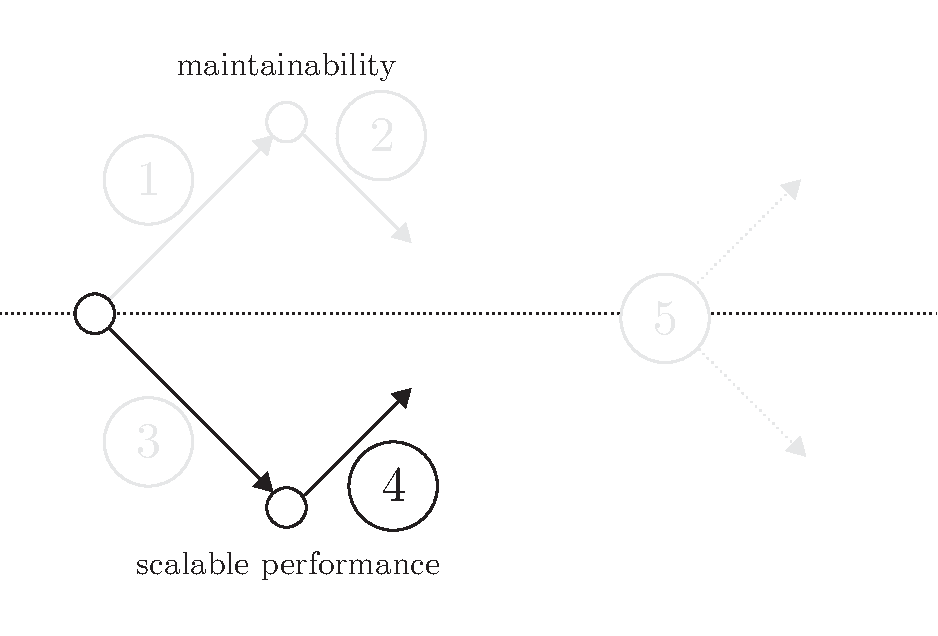
\includegraphics[width=0.6\textwidth]{../ressources/state-of-the-art-4.pdf}
\end{center}
\caption{}
\label{fig:state-of-the-art-4}
\end{figure}

The performance improvements comes directly from the industry requirements.
All these system make sens in industrial context, even the smallest.
When the need for performance is higher than the need for maintainability, the research merges with the academy.
% Industries have the money to fund the necessary research.
If there is industrial need, there will be maintenance.
The languages on the Mars Rover or in banking systems are 30 years old, and there is no community to maintain it.
Yet the industry continue to maintain these languages.

However, the context of this thesis is different from a classical industrial context.
During the bootstrap of a web application project, the economical context requires technologies with strong community, to pick talents from to grow the team quickly and effortlessly.
It also requires these technologies to be of industrial standard, to build a reliable product.
And these technology must be compatible with web technologies.

The context of this thesis requires the technology to meet all the three criteria.
\begin{itemize}
\item Community support
\item Industrial need
\end{itemize}


\nt{review this paragraph and the transition to the next section}
The field of concurrent programming is so vast it is impossible to relate here every programming languages.
The previous examples are only the best known.
The next focus focuses on streaming real-time applications.

% \comment{transition on lazy evaluation equivalence to stream. lazy evaluation + side effects + concurrency = streams}



% + all the solutions that have a great industrial impact (storm, millwheel and co)



\subsubsection{Exection Decomposition}


The programming paradigms presented above are implemented in many existing programming languages.
All major programming languages implements some form of concurrency or parallelism mechanism.
The next paragraphs presents these implementations by the industry and the community.
And more specifically, how they deal with the need to decompose the execution.

\paragraph{Event-Loop}

The event-loop model, featured by the DOM and Node.js with Javascript, allows concurrency but not parallelism.
It decomposes the execution into sequences of callbacks functions, but keep the memory shared.

As presented in the previous section, Javascript is currently one of the most used language.
This asynchronous programming model without the memory decomposition seems to be easy to develop with.
It is used extensively in the community as well as in the industry.
However, when the programming model requires the memory to be decompose, in order to get parallelism, it becomes more complicated to develop with, as presented in the next paragraphs.

\paragraph{Multi-Threading}

The multi-threading model allows concurrency and parallelism on certain execution region.
It decomposes the execution into fork-join threads, and the memory is shared, but protected with locks.
The protection of the shared memory is the reason concurrent programming is difficult to manage for most developers.
Multi-threading is difficult to program with, and for this reason, it leads to poor performances.
It is not heavily used in the community, where the need for concurrency is limited.
In the industry, where the concurrency is often required, multi-threading is abandoned for other paradigms, such as the event loop or the actor model.

\paragraph{}

The event-loop requires an execution decomposition, but not a memory decomposition.
This paradigm is heavily adopted by both the community and the industry.
On the other hand, the multi-threading paradigms with locks requires an execution decomposition, and light memory decomposition.
This paradigms is not heavily used in the community, and is being abandoned by the industry.
This comparison between the event-loop and the multi-threading paradigms seems to indicate that the memory decomposition heavily restrains the adoption by the community.
Hence, it impacts the maintainability required for the adoption in the economical context of this thesis, as shown in table \ref{scalability-execution-decomposition}.

\begin{table}[h!]
\label{scalability-execution-decomposition}
\small
\begin{tabu} to \linewidth {@{} l X[l] c c c c @{}}
%
% \multicolumn{3}{c}{}  & \lab{Concurrency} & \multicolumn{2}{|c}{Parallelism} \\
Model & Implementations    & \lab{Community adoption} & \lab{Industrial adoption} & $\to$ & \lab{Adoption} \\
\tabucline[.5pt]{-}
% %                                                                             COM  IND   GRO
Event-driven programming       & Node.js, Vert.X                               & \V & \V && \V \\ \tabucline[on .5pt]{-}
Multi-threading programming    & Lock, Mutex, Semaphores, Guarded regions      & \X & \V && \X \\
\tabucline[.5pt]{-}
\end{tabu}
\caption{Analysis of the state of the art in concurrent programming regarding adoption}
\end{table}

The next paragraphs present solutions that forces both the execution and memory decomposition to allow parallel execution.

\subsubsection{Actor Model}

The theoretical models presented in section \ref{chapter3:software-performance:parallel-programming} are implemented in industrial languages.
Example of implementation are Akka Scala and Erlang \cite{JoeArmstrong}.

Scala is an attempt at unifying the object model, and functional programming \cite{Odersky2004}.
It proposes an actor approach in its design.
Akka\ftnt{http://akka.io/} is a framework based on Scala, following the actor model to build highly scalable and resilient applications.
Play\ftnt{https://www.playframework.com/} is a web framework based on top of Akka.

Erlang borrow the Actor model as well.
It is a functional concurrent language designed by Ericsson to operate telecommunication devices \cite{Armstrong1993,Nelson2004}
% Nelson2004 is not very good, find another better citation.

These two example of implementation are heavily used in the industry.
They are backed by strong, but small communities of passionate people, as the actor model is not trivial to understand.

Moreover, the actor model decomposes the execution into isolated parallel executions, and the memory into independent stores.
These decompositions are hardly compatible with the modularity programming presented in the previous section.
It is difficult for developers to manage these decompositions, executions and memory, and the modularity of the implementation.
It restrain the maintainability of the implementation.
Most developers are unable to manage efficiently the two decompositions required by the actor model.
And novice developers seems reluctant to learn it.
The next paragraphs presents some solutions based on the actor model, with the intent to mitigate the duality between execution decomposition and modularity.

\paragraph{Design Patterns}

To reduce the difficulties of the decomposition of the execution into actors, algorithmic skeletons propose predefined patterns that fit certain type of problems \cite{Cole1988, Dean2008, McCool2010, Gonzalez-Velez2010}.
A developer implements the problem as a specific case of a skeleton.
It simplifies the communications, so that the developer can focus on its problem independently of message passing required by the distribution of execution.
These solutions are hardly used by the community, but are crucial in industrial contexts.
A famous example in the industry is map/reduce, introduce by Google \cite{Dean2008}.

% \nt{Link with DSMS}
% As there is similtudes between SQL-like languages, functional structures, and algorithmic skeletons, the latter can be seen as a tentative to merge the more descriptional features of the former into imperative programming.
% Indeed, among the Algorithmic skeletons, we can cite Map / reduce, which are functional structures, but are somehow equivalent to the select and aggregate functions of SQL.
% The pipeline architecture for data stream processing presented in section \ref{chapter3:software-efficiency:dataflow-pipeline} can be considered as algorithmic skeletons.

% However, they introduce limitations and difficulties, as the developer must fit its problem into the skeletons.
% One of this difficulties, it that a common memory is impossible to use.
% Developers needs to think in terms of message passing instead of a global memory, which, as we saw in previous section, is incompatible with best practices.

% Introducing 'Bones': a parallelizing source-to-source compiler based on algorithmic skeletons \cite{Nugteren2012}

\paragraph{Granularity}

The Service Oriented Architectures (SOA), and more recently Microservice\cite{Namiot2014,Fernandez-Villamor2010,Fowler2014,Namiot2014} allow developers to express an application as an assembly of services connected to each others.
Some examples of frameworks are OSGi\ftnt{https://www.osgi.org/developer/specifications/}, EJB\ftnt{http://www.oracle.com/technetwork/java/javaee/ejb/index.html}, Spring\ftnt{http://projects.spring.io/spring-framework/}, and Seneca\ftnt{http://senecajs.org/}
It intends to adjust the granularity of execution decomposition to help developers to fit the two organizations, the modular organization and the parallel execution organization \cite{Adam2008}.
Microservices are very recent, and it is difficult to asses their usage in the community nor the industry.
But they seems to be increasingly adopted, both in the industry and in the community.

% In modular programming a module protects the rest of the implementation from the consequences of the design choice its encapsulate, while a service encapsulate a specific task, with possible consequences on the adjacent services.

% In a fine enough granularity of service, each service becomes so simple, it can limits the consequences of its modification.


\subsubsection{Stream Processing Systems}

All the solutions previously presented are designed to build general distributed systems.
In the context of the web, a real-time application must process high volumes streams of requests within a certain time.
Because these systems are key to business, their reliability and latency are of critical importance.
Otherwise, input data may be lost or output data may lose their value.
These requirements are challenging to meet in the design of such system.

\paragraph{Data-stream Management Systems}

Database Management Systems (DBMS) historically processed large volume of data, and they naturally evolved into Data-stream Management System (DSMS) to processed data streams as well.
Because of this evolution, they are in rupture with imperative languages presented until now, and borrow the syntax from SQL.

DSMS concurrently run SQL-like requests on continuous data streams.
The computation of these requests spread over a distributed architecture.
Among the early works, we can cite
NiagaraCQ \cite{Chen2000,Naughton2001},
Aurora \cite{Abadi2003,Abadi2003a,Balakrishnan2004} which evolved into
Borealis \cite{Abadi2005},
AQuery \cite{Lerner2003},
STREAM \cite{Arasu2003,Arasu2005} and
TelegraphCQ \cite{Krishnamurthy2003,Chandrasekaran2003}.
More recently, we can cite
DryadLINQ \cite{Isard2007,Yu2009},
Apache Hive \cite{Thusoo2009}\ftnt{https://hive.apache.org/},
Timestream \cite{Qian2013} and
Shark \cite{Xin2013}.


\paragraph{Pipeline Architecture}

As presented in the previous section, streaming and lazy-evaluation composition both allow a loosely coupled yet efficient composition.
The pipeline architecture takes advantage of this, and composes the parallel execution in a stream, the output of one feeding the input of the next.

SEDA is a precursor in the design of pipeline-based architecture for real-time web applications \cite{Welsh2001}.
It organizes an application as a network of event-driven stages connected by explicit queues.
The event-driven paradigm is similar to previous web servers implementations like Ninja and Flash \cite{Gribble2001,Pai1999}.
SEDA improves with the pipeline organization in stages.

Several projects followed and adapted the principles in this work.
StreaMIT is a language to help the programming of large streaming application \cite{Thies2002}.
Storm \cite{Toshniwal2014} is designed by and used at Twitter to process the heavy streams of tweets.
% It is only one example of industrial practical application, among many others.
Among other works, in the industry, there are
CBP \cite{Logothetis2010} and
S4 \cite{Neumeyer2010}, that were designed at Yahoo,
Millwheel \cite{Akidau2013} designed at Google and
Naiad \cite{Murray2013} designed at Microsoft.

In the litterature, there are
Spidle \cite{Consel2003},
Pig Latin \cite{Olston2008},
Piccolo \cite{Power2010},
Comet \cite{He2010},
Nectar \cite{Gunda2010},
SEEP \cite{Migliavacca2010},
Legion \cite{Bauer2012},
Halide \cite{Ragan-Kelley2013},
SDG \cite{Fernandez2014a} and
Regent \cite{Slaughter2015}


\paragraph{}

At the light of this analysis, it appears that parallel programming is not heavily adopted by the community.
The execution decomposition required by parallel programming improve performance scalability, but reduce the adoption required for maintainability.
Eventually, only the event-loop is a viable concurrent programming approach in the economical context of the web.
And it is exactly what the numbers indicates through the heavy adoption of Javascript in the last few years.

\begin{table}[h!]
\label{scalability-growth}
\small
\begin{tabu} to \linewidth {@{} l X[l] c c c c c @{}}
%
% \multicolumn{3}{c}{}  & \lab{Concurrency} & \multicolumn{2}{|c}{Parallelism} \\
Model & Implementations    & \lab{Community adoption} & \lab{Industrial adoption} & \lab{Web compliant} & $\to$ & \lab{Adoption} \\
\tabucline[.5pt]{-}
% %                                                                               COM  IND  WEB   GRO
Event-driven programming       & Node.js, Vert.X                               & \V & \V & \V && \V \\ \tabucline[on .5pt]{-}
Multi-threading programming    & Lock, Mutex, Semaphores, Guarded regions      & \X & \V & \V && \X \\ \tabucline[on .5pt]{-}
Lock-free Data Structures      &                                               & \X & \V & \V && \X \\
\tabucline[.5pt]{-}
Actor Model                    & Scala, Akka, Play, Erlang                     & \M & \V & \V && \M \\ \tabucline[on .5pt]{-}
Skeleton                       & MapReduce, ...                                & \X & \V & \V && \X \\ \tabucline[on .5pt]{-}
Service Oriented Architecture  & OSGi, EJB, Spring                             & \J & \V & \V && \J \\ \tabucline[on .5pt]{-}
Microservices                  & Seneca                                        & \U & \U & \V && \U \\
\tabucline[.5pt]{-}
Data Stream System Management  & DryadLINQ \cite{Isard2007,Yu2009},%
                                 Apache Hive \cite{Thusoo2009}\ftnt{https://hive.apache.org/},%
                                 Timestream \cite{Qian2013},%
                                 Shark \cite{Xin2013}.                         & \X & \V & \V && \X \\ \tabucline[on .5pt]{-}
Pipeline Stream Processing     & SEDA, Storm, Spark Streaming,%
                                 Spidle \cite{Consel2003},%
                                 Pig Latin \cite{Olston2008},%
                                 Piccolo \cite{Power2010},%
                                 Comet \cite{He2010},%
                                 Nectar \cite{Gunda2010},%
                                 SEEP \cite{Migliavacca2010},%
                                 Legion \cite{Bauer2012},%
                                 Halide \cite{Ragan-Kelley2013},%
                                 SDG \cite{Fernandez2014a},%
                                 Regent \cite{Slaughter2015}.                  & \X & \V & \V && \X \\
\tabucline[.5pt]{-}
\end{tabu}
\caption{Analysis of the state of the art in concurrent and parallel programming regarding adoption}
\end{table}

\subsection{Maintainability Limitations} \label{chapter3:software-performance:maintainability-limitations}

Parallel programming requires the decomposition of memory and execution to allow the different levels of state accessibility and execution.
At a fine level, the state is shared, while at a coarser level, it is isolated.
Because of this decomposition, programming languages abandoned shared state, and higher-order programming between execution containers.

Indeed, the topology of the network of actors is statically defined, and the dynamical modification of the topology is mostly impossible.
It is not possible to dynamically manipulate execution containers, like it is possible to manipulate functions.
Therefore, higher-level programming is impossible, and limits the modularity required for maintainability.
It implies to keep two mental representation of the implementation, one for the modularity, and one for the decomposition of execution.
Parallel programming remains hard, and is accessible only to an elite of developers.
In this regards, the memory decomposition required by parallel programming is incompatible with the economical context required in this thesis.

To fit the economical context of this thesis, a solution must provide scalability, hence memory and execution decomposition.
But at the same time proposes an abstraction for the memory decomposition, to avoid the developers to keep a double mental representation of the implementation.
The next section presents some works that provides such a memory decomposition abstraction.

\begin{table}[h!]
\label{scalability-maintainability}
\small
\begin{tabu} to \linewidth {@{} l X[l] c c c @{}}
%
% \multicolumn{3}{c}{}  & \lab{Concurrency} & \multicolumn{2}{|c}{Parallelism} \\
Model & Implementations    & \lab{Memory decomposition abstraction} & $\to$ & \lab{Maintainability} \\
\tabucline[.5pt]{-}
%                                                                               ABS   MAI
Event-driven programming       & Node.js, Vert.X                               & \V && \V \\ \tabucline[on .5pt]{-}
Lock-free Data Structures      &                                               & \X && \X \\ \tabucline[on .5pt]{-}
Multi-threading programming    & Lock, Mutex, Semaphores, Guarded regions      & \X && \X \\
\tabucline[.5pt]{-}
Actor Model                    & Scala, Akka, Play, Erlang                     & \X && \X \\ \tabucline[on .5pt]{-}
Skeleton                       & MapReduce, ...                                & \X && \X \\ \tabucline[on .5pt]{-}
Service Oriented Architecture  & OSGi, EJB, Spring                             & \X && \X \\ \tabucline[on .5pt]{-}
Microservices                  & Seneca                                        & \X && \X \\
\tabucline[.5pt]{-}
Data Stream System Management  & DryadLINQ \cite{Isard2007,Yu2009},%
                                 Apache Hive \cite{Thusoo2009}\ftnt{https://hive.apache.org/},%
                                 Timestream \cite{Qian2013},%
                                 Shark \cite{Xin2013}.                         & \X && \X \\ \tabucline[on .5pt]{-}
Pipeline Stream Processing     & SEDA, Storm, Spark Streaming,%
                                 Spidle \cite{Consel2003},%
                                 Pig Latin \cite{Olston2008},%
                                 Piccolo \cite{Power2010},%
                                 Comet \cite{He2010},%
                                 Nectar \cite{Gunda2010},%
                                 SEEP \cite{Migliavacca2010},%
                                 Legion \cite{Bauer2012},%
                                 Halide \cite{Ragan-Kelley2013},%
                                 SDG \cite{Fernandez2014a},%
                                 Regent \cite{Slaughter2015}.                  & \X && \X \\
\tabucline[.5pt]{-}
\end{tabu}
\caption{Analysis of the state of the art regarding maintainability}
\end{table}


\subsection{Summary} \label{chapter3:software-performance:summary}

Table \ref{scalability-synthesis} summarizes the characteristics of the solutions presented in this section.

\begin{table}[h!]
\label{scalability-synthesis}
\small
\begin{tabu} to \linewidth {@{} l X[l] c c c @{}}
%
% \multicolumn{3}{c}{}  & \lab{Concurrency} & \multicolumn{2}{|c}{Parallelism} \\
Model & Implementations    & \lab{Maintainability} & \lab{Adoption} & \lab{Performance Efficiency} \\
\tabucline[.5pt]{-}
%                                                                               MAI  GRO  SCA
Event-driven programming       & Node.js, Vert.X                               & \V & \V & \X \\ \tabucline[on .5pt]{-}
Lock-free Data Structures      &                                               & \X & \V & \V \\ \tabucline[on .5pt]{-}
Multi-threading programming    & Lock, Mutex, Semaphores, Guarded regions      & \X & \V & \V \\
\tabucline[.5pt]{-}
Actor Model                    & Scala, Akka, Play, Erlang                     & \X & \M & \V \\ \tabucline[on .5pt]{-}
Skeleton                       & MapReduce, ...                                & \X & \X & \V \\ \tabucline[on .5pt]{-}
Service Oriented Architecture  & OSGi, EJB, Spring                             & \X & \J & \V \\ \tabucline[on .5pt]{-}
Microservices                  & Seneca                                        & \X & \X & \V \\
\tabucline[.5pt]{-}
Data Stream System Management  & DryadLINQ \cite{Isard2007,Yu2009},%
                                 Apache Hive \cite{Thusoo2009}\ftnt{https://hive.apache.org/},%
                                 Timestream \cite{Qian2013},%
                                 Shark \cite{Xin2013}.                         & \X & \X & \V \\ \tabucline[on .5pt]{-}
Pipeline Stream Processing     & SEDA, Storm, Spark Streaming,%
                                 Spidle \cite{Consel2003},%
                                 Pig Latin \cite{Olston2008},%
                                 Piccolo \cite{Power2010},%
                                 Comet \cite{He2010},%
                                 Nectar \cite{Gunda2010},%
                                 SEEP \cite{Migliavacca2010},%
                                 Legion \cite{Bauer2012},%
                                 Halide \cite{Ragan-Kelley2013},%
                                 SDG \cite{Fernandez2014a},%
                                 Regent \cite{Slaughter2015}.                  & \X & \X & \V \\
\tabucline[.5pt]{-}
\end{tabu}
\caption{Summary of the analysis of the state of the art in concurrent and parallel programming}
\end{table}

\endinput







TO READ :

Streaming
\cite{Madsen2015}
\cite{Sun2015}

Map Reduce
\cite{Yao2015}


Web assembly
https://medium.com/javascript-scene/what-is-webassembly-the-dawn-of-a-new-era-61256ec5a8f6












\endinput

\subsection{Concurrency Theory} \label{chapter3:parallel-execution:concurrency-theory}

The mathematical models are a ground for all following work on concurrent programming, we briefly explain them in the next paragraphs.
There are two main formal models for concurrent computations.
The Actor Model of C. Hewitt and the Pi-calculus of R. Milner.
Based on these definitions, we explain the importance of determinism for correctness, and the reasons that made asynchronous message-passing prevail.

% TODO illustration of cells, and draw an analogy between cells and actor model.
% Or something the actor models is based upon.

\subsubsection{Models}

\paragraph{Actor Model}

The Actor model allows to express the computation as a set of communicating actors \cite{Hewitt1973a, Hewitt1977, Clinger1981}.
In reaction to a received message, an actor can create other actors, send messages, and choose how to respond to the next message.
All actors are executed concurrently, and communicate asynchronously.
% The Actor model uses an asynchronous message-passing communication paradigm.
% The communication between two actors, the sender and the receiver, is a stream of discrete messages.
% The sender names the receiver actor when sending messages to be the recipient of these messages.
An asynchronous communication implies that the sender continues its execution immediately after sending the message, before receiving the result of the initiated communication.

The Actor model was presented as a highly parallel programming model, but intended for Artificial Intelligence purposes.
Its success spread way out of this scope, and it became a general reference and influence.
% For example, the Scala programming language features an actor approach to concurrency.

% More recent work of C. Hewitt on Actors is about ... \nt{TODO} \cite{Hewitt2007,Hewitt2007a}.

\paragraph{$\pi$-calculus}

R. Milner presented a process calculus to describe concurrent computation : the Calculus of Communicating Systems (CCS) \cite{Milner1975, Milner1980}.
It is an algebraic notation to express identified processes communicating through synchronous labeled channels.
% In CCS, process compose concurrently, communications are synchronous, and the topology is static.
The $\pi$-calculus improved upon this earlier work to allow processes to be communicated as values, hence to become mobile \cite{Engberg1986,Milner1992a,Milner1992}.
Therefore, similarly to Actors, in Pi-calculus processes can dynamically modify the topology.
However, contrary to the Actor model, communications in Pi-calculus are based on simultaneous execution of complementary actions, they are synchronous.


% Actors can create actors, pi-caclulys processes can replicate, and send processes through channel.
% Processes create a new processes on each instruction to continue the execution.!g systolic arrays

% Pi-calculus resembles to the actor model, but its algebraic nature led to a critical difference with the latter.
% Indeed, processes in the Pi-calculus communicate indirectly, through labeled ports, whereas actors communicate directly by naming the recipient actors.
% This difference allows multiple processes to listen in turns to the same channel, whereas the recipient of a message cannot change.

% I think this difference lead the Pi-calculus to be composable, whereas message-passing is not.
% Message-passing is not composable, whereas invocation is.
% The Actor model is not an ideal programming model, as non-composability makes difficult to reuse or extends existing components.
% A way to compose actors, is to send to an actor the name of the actor to respond to.
% It is similar in essence to the continuation concept.








\section{Reconciliations} \label{chapter3:reconciliations}
\nt{TODO title not clear enough}

\subsection{Contradiction}

The decomposition of an application into a pipeline, as shown in the two previous sections, is incompatible with the modular design advocated by the separation of concerns.
The problem of incompatibility between the modular design and the parallel execution of a pipeline architecture is the following.
There need to be a common understanding on the structure of the communication from one stage to the next.
The modular design defines that this common ground, the interface, be the most resilient possible to focus the evolution within a module.
While the pipeline architecture (and more generally the concurrent programming models) defines these interfaces as the communications between the stages of the execution.
With the evolution of the problem specification, when a stage needs to be modified, it is most likely that these changes will affect the previous or next stages.
% which will eventually change with the evolution of the problem specification.

Most project use languages supporting the modular design at the beginning, when they need to evolve the most.
They then switch to the pipeline architecture only when the requirement of performance overcomes the requirement of evolution.
Moreover, as the team knows that they will eventually throw away their code to upgrade it to a different paradigm, there is little effort to follow the best practice to make maintainable code.
It results in a large effort of development to compensate this rupture.
% This rupture between the two organization is not novel, and is at the center of a large body of work.
In this section, we present the state of the art to reconciliate the two organizations, and avoid this rupture.
First we see the design patterns to fit both organization onto a same source code.
Then we see the compilation tentatives to switch from one to the other.